\section{\begin{CJK}{UTF8}{gkai}
		MapReduce介绍
\end{CJK}}

\subsection{\begin{CJK}{UTF8}{gkai}什么是MapReduce?
\end{CJK}}

\begin{frame}{\begin{CJK}{UTF8}{gkai}提出背景
			\end{CJK}}
	\begin{columns}
		\begin{column}{0.5\textwidth}
			\begin{itemize}
				\item \begin{CJK}{UTF8}{gkai}
					2003年和2004年,Google分别发表了两篇关于Google分布式文件系统和MapReduce的论文。\end{CJK}
				\item \begin{CJK}{UTF8}{gkai}
				Google公司设计MapReduce的初衷主要是为了\alert{解决其搜索引擎中大规模网页数据的并行化处理}。\end{CJK}
				\item \begin{CJK}{UTF8}{gkai}MapReduce其后被广泛应用于众多大规模数据处理问题。\end{CJK}
			\end{itemize}
		
		\end{column}
		
		\begin{column}{0.5\textwidth}
			\centerline{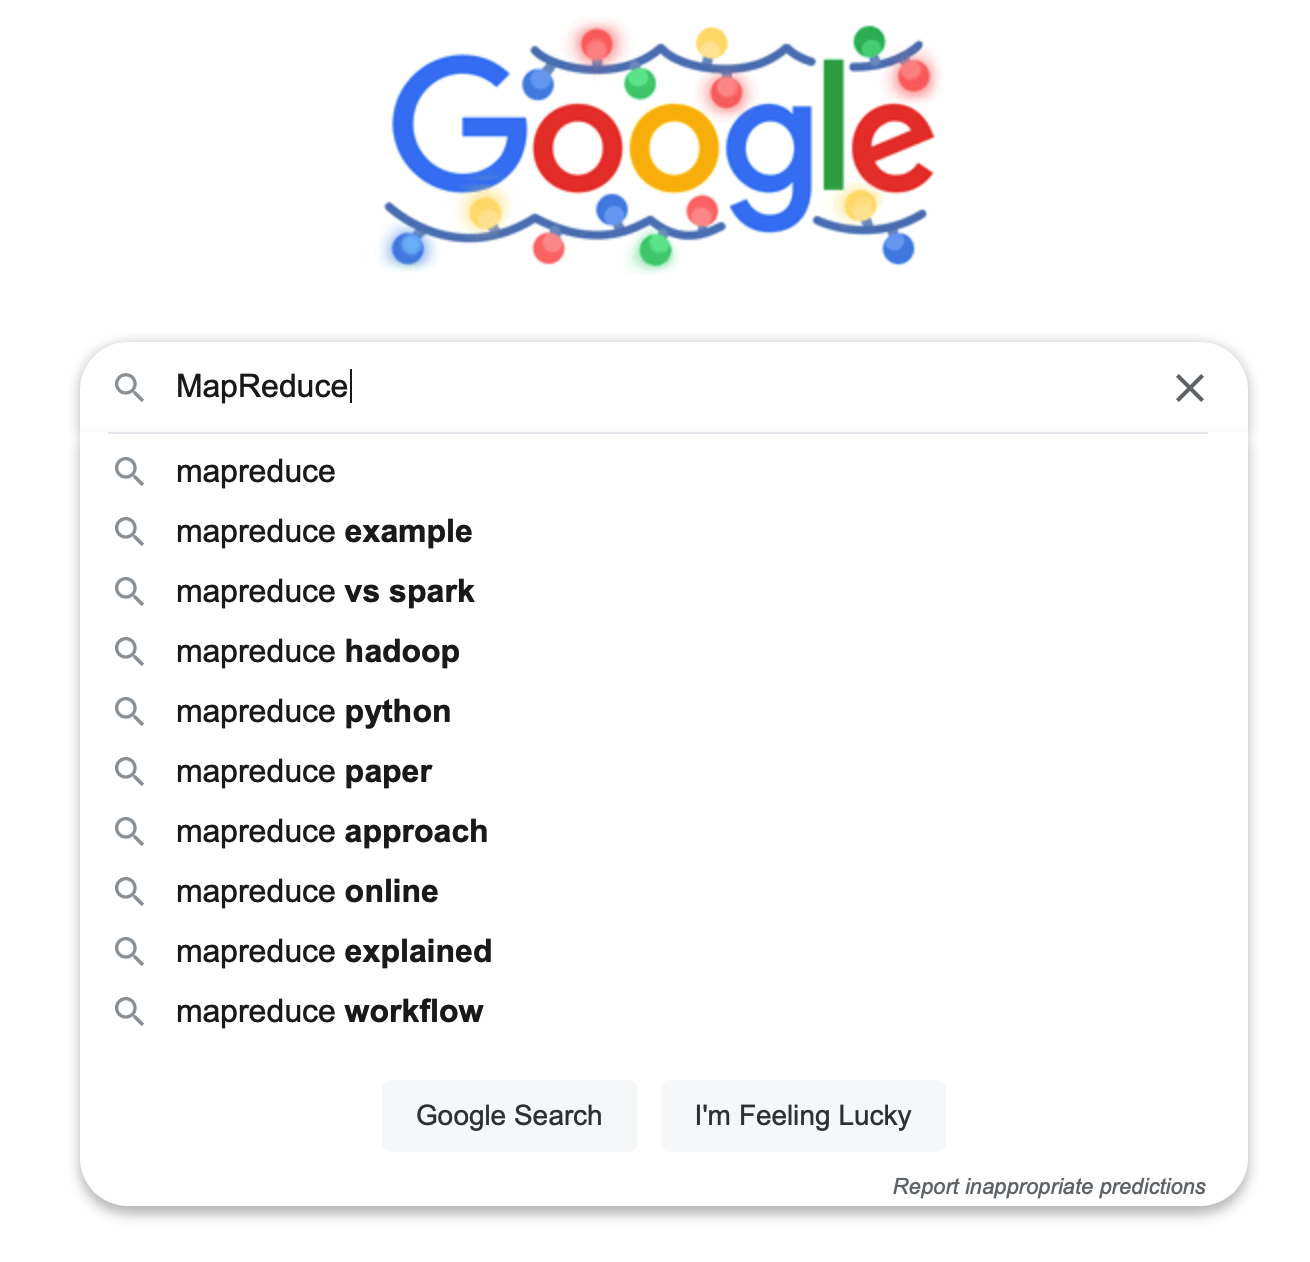
\includegraphics[width = 0.9\textwidth]{Figures/google.png}}
			\centerline{https://www.google.com}
		\end{column}
	\end{columns}
\end{frame}

\begin{frame}{\begin{CJK}{UTF8}{gkai}相关文献
	\end{CJK}}
	\centerline{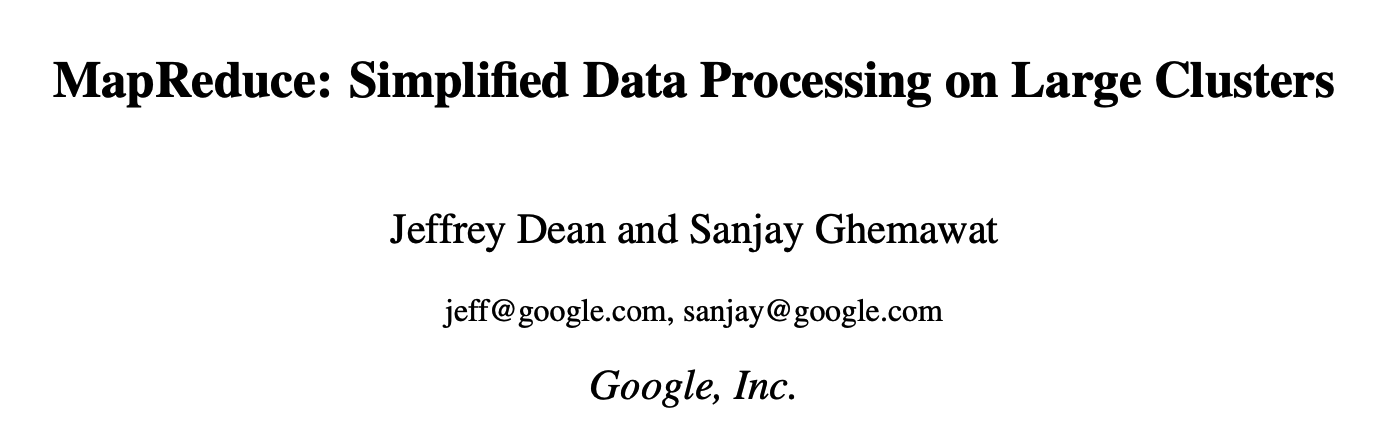
\includegraphics[width = 0.9\textwidth]{Figures/ref.png}}
	Abstract:
	\begin{itemize}
		\item MapReduce is a programming model and an associated implementation for \alert{processing and generating large data sets}.
		\item Upwards of one thousand MapReduce jobs are executed on Google’s clusters every day.
	\end{itemize}
\end{frame}

\begin{frame}{\begin{CJK}{UTF8}{gkai}思想由来
	\end{CJK}}
	\begin{alertblock}{Abstract}
		Our abstraction is inspired by the map and reduce primitives present in Lisp and many other functional languages.\\
		\rightline{\begin{CJK}{UTF8}{gkai}————Google, Inc.
		\end{CJK}}\\
		\
		\newline\\
		
		\begin{CJK}{UTF8}{gkai}此即MapReduce的思想渊源,简言之,MapReduce的灵感来源于函数式语言(比如Lisp)中的内置函数map和reduce。\end{CJK}
	\end{alertblock}
	
	\begin{CJK}{UTF8}{gkai}在函数式语言里:
	\end{CJK}
	\begin{description}
		\item[map] \begin{CJK}{UTF8}{gkai}表示对一个列表(List)中的每个元素做计算;
		\end{CJK}
		\item[reduce] \begin{CJK}{UTF8}{gkai}表示对一个列表中的每个元素做迭代计算。
		\end{CJK}
	\end{description}
	\begin{CJK}{UTF8}{gkai}它们具体的计算是通过传入的函数来实现的,map和reduce提供的是计算的框架。
	\end{CJK}
	
\end{frame}

\begin{frame}{\begin{CJK}{UTF8}{gkai}思想发展
	\end{CJK}}
	\begin{CJK}{UTF8}{gkai}依据Map与Reduce各自的内涵,我们可以把MapReduce理解为如下几个过程:
	\end{CJK}
	\begin{description}
		\item[map] \begin{CJK}{UTF8}{gkai}提取特征:\\
			面对的是杂乱无章的互不相关的数据,它解析每个数据,从中提取出key和value,也就是提取了数据的特征;
		\end{CJK}
		\item[shuffle] \begin{CJK}{UTF8}{gkai}依据某种特征归纳数据;\end{CJK}
		\item[reduce] \begin{CJK}{UTF8}{gkai}处理并得到最后的结果。
		\end{CJK}
	\end{description}
	
	\begin{block}{Hadoop}
		\begin{CJK}{UTF8}{gkai}
			一个基于Java设计开发的开源MapReduce并行计算框架和系统,由开源项目Lucene(搜索索引程序库)和Nutch(搜索引擎)的创始人Doug Cutting模仿Google MapReduce所编写。
			
		\end{CJK}
	\end{block}
	
\end{frame}

\begin{frame}{\begin{CJK}{UTF8}{gkai}
			MapReduce定义
			\end{CJK}}
	\cite[pp.~74--75]{MapReduce}
	\begin{definition}
		\begin{enumerate}
			\item \begin{CJK}{UTF8}{gkai}
				一种数据并行模型,用于大规模数据集(大于1TB)的并行运算;\end{CJK}
			\item \begin{CJK}{UTF8}{gkai}采用\alert{"分而治之"}的思想,把对大规模数据集的操作,分发给一个主节点管理下的各个分节点共同完成,然后通过整合各个节点的中间结果,得到最终结果;\end{CJK}
			\item \begin{CJK}{UTF8}{gkai}然后通过整合各个节点的中间结果,得到最终结果。\end{CJK}
		\end{enumerate}
		
	\end{definition}
	\begin{CJK}{UTF8}{gkai}在分布式计算中,MapReduce框架负责处理了并行编程中分布式存储、工作调度、负载均衡、容错均衡、容错处理以及网络通信等复杂问题,把处理过程高度抽象为两个函数:Map和Reduce。\end{CJK}
	
\end{frame}

\begin{frame}{\begin{CJK}{UTF8}{gkai}
			图片示意
	\end{CJK}}
	
	\begin{columns}
		\begin{column}{0.5\textwidth}
			\centerline{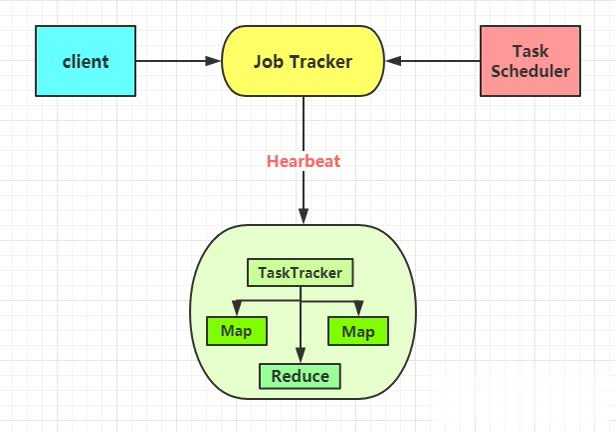
\includegraphics[width = 1.1\textwidth]{Figures/ll.jpg}}
			\centerline{\begin{CJK}{UTF8}{gkai}
					MapReduce架构图
			\end{CJK}}
		\end{column}
		
		\begin{column}{0.5\textwidth}
			\begin{description}
				\item[client] \begin{CJK}{UTF8}{gkai}用于提交任务;
				\end{CJK}
				\item[Job Tracker
				] \begin{CJK}{UTF8}{gkai}负责资源监控和作业调度;
				\end{CJK}
				\item[map] \begin{CJK}{UTF8}{gkai}负责把任务分解成多个任务;
				\end{CJK}
				\item[reduce] \begin{CJK}{UTF8}{gkai}Reduce负责把分解后多任务处理的结果汇总起来。
				\end{CJK}
			\end{description}
			
		\end{column}
		
		
	\end{columns}

\end{frame}
